% This must be in the first 5 lines to tell arXiv to use pdfLaTeX, which is strongly recommended.
\pdfoutput=1
% In particular, the hyperref package requires pdfLaTeX in order to break URLs across lines.

\documentclass[11pt]{article}

% Change "review" to "final" to generate the final (sometimes called camera-ready) version.
% Change to "preprint" to generate a non-anonymous version with page numbers.
%\usepackage[review]{acl}
\usepackage{gb4e}
\noautomath
\usepackage{acl}

% Standard package includes
\usepackage{times}
\usepackage{latexsym}


% For proper rendering and hyphenation of words containing Latin characters (including in bib files)
\usepackage[T1]{fontenc}
% For Vietnamese characters
% \usepackage[T5]{fontenc}
% See https://www.latex-project.org/help/documentation/encguide.pdf for other character sets

% This assumes your files are encoded as UTF8
\usepackage[utf8]{inputenc}

% This is not strictly necessary, and may be commented out,
% but it will improve the layout of the manuscript,
% and will typically save some space.
\usepackage{microtype}

% This is also not strictly necessary, and may be commented out.
% However, it will improve the aesthetics of text in
% the typewriter font.
\usepackage{inconsolata}

%Including images in your LaTeX document requires adding
%additional package(s)
\usepackage{graphicx}

% If the title and author information does not fit in the area allocated, uncomment the following
%
%\setlength\titlebox{<dim>}
%
% and set <dim> to something 5cm or larger.

\newcommand{\todo}[1]{\textcolor{red}{(\textbf{TODO:} #1)}}
\newcommand{\goldmant}{\citet{goldman-etal-2022-un}}
\newcommand{\goldmana}{\citeauthor{goldman-etal-2022-un}}
\newcommand{\goldmanp}{\citep{goldman-etal-2022-un}}

\newcommand{\kodnert}{\citet{kodner-etal-2022-sigmorphon}}
\newcommand{\kodnera}{\citeauthor{kodner-etal-2022-sigmorphon}}
\newcommand{\kodnerp}{\citep{kodner-etal-2022-sigmorphon}}

\title{Evaluating Evaluation: Comparing Adversarial Approaches to Evaluating Neural Models of Morphological Inflection}

% Author information can be set in various styles:
% For several authors from the same institution:
% \author{Author 1 \and ... \and Author n \\
%         Address line \\ ... \\ Address line}
% if the names do not fit well on one line use
%         Author 1 \\ {\bf Author 2} \\ ... \\ {\bf Author n} \\
% For authors from different institutions:
% \author{Author 1 \\ Address line \\  ... \\ Address line
%         \And  ... \And
%         Author n \\ Address line \\ ... \\ Address line}
% To start a separate ``row'' of authors use \AND, as in
% \author{Author 1 \\ Address line \\  ... \\ Address line
%         \AND
%         Author 2 \\ Address line \\ ... \\ Address line \And
%         Author 3 \\ Address line \\ ... \\ Address line}

\author{Sarah Payne, QP2 Proposal\\
  Stony Brook University \\
  \texttt{sarah.payne@stonybrook.edu} }

%\author{
%  \textbf{First Author\textsuperscript{1}},
%  \textbf{Second Author\textsuperscript{1,2}},
%  \textbf{Third T. Author\textsuperscript{1}},
%  \textbf{Fourth Author\textsuperscript{1}},
%\\
%  \textbf{Fifth Author\textsuperscript{1,2}},
%  \textbf{Sixth Author\textsuperscript{1}},
%  \textbf{Seventh Author\textsuperscript{1}},
%  \textbf{Eighth Author \textsuperscript{1,2,3,4}},
%\\
%  \textbf{Ninth Author\textsuperscript{1}},
%  \textbf{Tenth Author\textsuperscript{1}},
%  \textbf{Eleventh E. Author\textsuperscript{1,2,3,4,5}},
%  \textbf{Twelfth Author\textsuperscript{1}},
%\\
%  \textbf{Thirteenth Author\textsuperscript{3}},
%  \textbf{Fourteenth F. Author\textsuperscript{2,4}},
%  \textbf{Fifteenth Author\textsuperscript{1}},
%  \textbf{Sixteenth Author\textsuperscript{1}},
%\\
%  \textbf{Seventeenth S. Author\textsuperscript{4,5}},
%  \textbf{Eighteenth Author\textsuperscript{3,4}},
%  \textbf{Nineteenth N. Author\textsuperscript{2,5}},
%  \textbf{Twentieth Author\textsuperscript{1}}
%\\
%\\
%  \textsuperscript{1}Affiliation 1,
%  \textsuperscript{2}Affiliation 2,
%  \textsuperscript{3}Affiliation 3,
%  \textsuperscript{4}Affiliation 4,
%  \textsuperscript{5}Affiliation 5
%\\
%  \small{
%    \textbf{Correspondence:} \href{mailto:email@domain}{email@domain}
%  }
%}

\begin{document}
\maketitle
\begin{abstract}
Morphological inflection is a fundamental task in subword NLP, popularized by the recent SIGMORPHON shared tasks. 
For several years now, state-of-the-art neural models have reported extremely high average accuracy across languages on these tasks. 
This apparent saturation has led to the development of a range of adversarial evaluation practices, based on the common insight that traditional train-test splits don't control for whether the model has seen either the \textit{lemma} or \textit{feature set} separately in its training data. 
These evaluation practices, however, differ drastically in their results: while \goldmant~ reports that models fail to generalize to unseen \textit{lemmas}, \kodnert~ find that the models have little trouble generalizing to unseen lemmas, but take a large performance hit when generalizing to unseen \textit{feature sets}. 
In this Qualifying Paper, I will \todo{}



\end{abstract}

\section{Introduction}

\todo{Write the Introduction \& maybe a related work section}

Generalization, the ability to extend patterns from known to unknown items, is a critical part of mor- phological competence. 
Morphological sparsity \todo{talk about sparsity and acquisition}

So far, the best-performing models have been neural sequence-to-sequence models \citep{kann-schutze-2016-med, canby-etal-2020-university}

Many subfields of NLP and machine learning in general suggested hard splits as means to improve the probing of models’ ability to solve the under- lying task, and to make sure models do not simply employ loopholes in the data.
The addition of unanswerable questions to question answering benchmarks \citep{rajpurkar-etal-2018-know}, or the addition of expert-annotated minimal pairs \citep{gardner-etal-2020-evaluating}. 
\citet{narayan-etal-2017-split} suggested using the \textsc{Websplit} data, where models are required to split and rephrase complex sentences associated with a meaning representation over a knowledge-base. 
\citet{aharoni-goldberg-2018-split} found that some facts appeared in both train and test sets and provided a harder split denying models the ability to use memorized facts. \citet{aharoni-goldberg-2020-unsupervised} also suggested a general splitting method for machine translation such that the domains are as disjoint as possible.
In semantic parsing, \citet{finegan-dollak-etal-2018-improving} suggested a better split for parsing natural language questions to SQL queries by making sure that queries of the same template do not occur in both train and test, while \citet{lachmy2022} split their HEXAGONS data such that any one visual pat- tern used for the task cannot appear in both train and test. 
Furthermore, \citet{loula-etal-2018-rearranging} adversarially split semantic parsing for navigation data to assess their models’ capability to use compositionality. In spoken language understanding \citet{arora2021} designed a splitting method that will account for variation in both speaker identity and linguistic content.



In general, concerns regarding data splits and their undesired influence on model assessments led \citet{gorman-bedrick-2019-need} to advocate random splitting instead of standard ones.
A common modification is re-splitting the data such that the test set is more challenging and closer to the intended use of the models in the wild \citep{sogaard-etal-2021-need}. As the performance on morphological inflection models seems to have saturated on high scores, a similar rethinking of the data used is warranted.

\textbf{Motivation for the generalization task:} 

\citet{pimentel-ryskina-etal-2021-sigmorphon} looked at lemma overlap as well but didn't control for featureset overlap 

\newpage
\section{Defining the Task}
\subsection{Morphological Inflection as an NLP Task}

In standard morphological inflection tasks, models are exposed to triples of \texttt{(lemma, feature set, inflected form)} during training.
During evaluation, the model is given a \texttt{(lemma, feature set)} pair as input and the goal is to correctly predict the corresponding inflected form.
For example,  were the model to be given as input (\texttt{walk}, \textsc{V;Past}), then we would expect it to output \texttt{walked}. 

\subsection{The Role of Overlap}
In most versions of the SIGMORPHON shared task \citep{cotterell-etal-2016-sigmorphon, cotterell-etal-2017-conll, cotterell-etal-2018-conll, mccarthy-etal-2019-sigmorphon, vylomova-etal-2020-sigmorphon, pimentel-ryskina-etal-2021-sigmorphon, goldman-etal-2023-sigmorphon}, train-test splits are created by randomly sampling from the available \texttt{(lemma, feature set, inflected form)} triples. 
While this approach entails that no triple occurring in the train set will occur in the evaluation set, as  both \goldmant~ and \kodnert~ note, it ignores the fact that lemmas or feature sets that appear during train may reappear during test, since lemmas and feature sets can be combined independently. 

To illustrate this point, consider the toy example below, taken from \citet{kodner-etal-2023-morphological}. 
Though none of the triples appearing in the train set (\ref{example-train}) re-appear in the evaluation set (\ref{example-test}), the lemmas and feature sets seen in train \textit{do} reappear individually in the evaluation set. 
For example, in \texttt{e0}, both the lemma and the feature set are attested separately in the training data: the lemma is attested in \texttt{t0} and the feature set is attested in \texttt{t1}. 
By contrast, in \texttt{e3}, neither the lemma nor the feature set are attested in the training data. 
Though neither \texttt{e0} nor \texttt{e3} are attested \textit{as entire triples} in the training data, one might expect that it would be easier for a model trained on (\ref{example-train}) to generate the correct result for \texttt{e0} than for \texttt{e3}. 



\begin{exe}
\ex\label{example-train} Example training set: \\
\begin{small}
\begin{tabular}{llll}
\texttt{t0:} & \texttt{see} & \texttt{seeing} & \textsc{V;V.Ptcp;Prs}\\
\texttt{t1:} & \texttt{sit} & \texttt{sat} & \textsc{V;Pst}\\
\end{tabular}
\end{small}
\ex\label{example-test} Example evaluation set:\\
\begin{small}
\begin{tabular}{lll}
\texttt{e0:} & \texttt{see} &  \textsc{V;Pst}\\
\texttt{e1:} & \texttt{sit} & \textsc{V;Nfin}\\
\texttt{e2:} & \texttt{eat} & \textsc{V;Pst}\\
\texttt{e3:} & \texttt{run} & \textsc{V;Prs;3;Sg}\\
\end{tabular}
\end{small}
\end{exe}

Indeed, this is the insight behind both \goldmant~ and \kodnert:  test pairs with novel lemmas or novel feature sets require a system to generalize along different morphological dimensions, and evaluation measures  should control for this overlap so as to better measure models' ability to generalize along these dimensions. 
To formalize these dimensions, \kodnert~ define four types of overlap, which we repeat here: 
\begin{itemize}
\item \textbf{\texttt{both} Overlap}: both the lemma and feature set of an evaluation pair are attested in train, though not together in the same triple (\texttt{e0} in example \ref{example-test})
\item \textbf{\texttt{lemmaOnly} Overlap}: only the lemma is attested in training, and the feature set is novel (\texttt{e1} in example \ref{example-test})
\item \textbf{\texttt{featsOnly} Overlap}: only the feature set is attested in training, and the lemma is novel (\texttt{e2} in example \ref{example-test})
\item \textbf{\texttt{neither} Overlap}: neither the lemma nor the feature set is attested in train (\texttt{e3} in example \ref{example-test})
\end{itemize} 

We additionally define \textbf{\texttt{featsAttested}} to be any evaluation triple for which the feature set is attested in train (i.e., \texttt{featsAttested} = \texttt{both} $\cup$ \texttt{featsOnly}) and \textbf{\texttt{featsNovel}} to be any evaluation triple for which the features are unattested in train (i.e. \texttt{featsNovel} = \texttt{lemmaOnly} $\cup$ \texttt{neither}). 
\textbf{\texttt{lemmaAttested}} and \textbf{\texttt{lemmaNovel}} are defined analogously. 



\section{Previous Work}

While most previous work on morphological inflection has made use of random train-test splits which do not control for overlap, two lines of work have examined different aspects of overlap. 
\citet[864]{goldman-etal-2022-un} focused on lemma overlap, arguing that models can short-cut their way to better predictions in cases where forms from the same lemma appear in both the train and test data" since the model may  be able to memorize lemma-specific irregularities.

Specifically, \goldmana~ propose an evaluation strategy in which train-test splits are formed by splitting by \textit{lemma} rather than by triple. 
As such, for any  lemma $\mathcal{L}$ in the data, all triples of the form \texttt{($\mathcal{L}$, feature set, inflected form)} are placed into the same set (either train or test); the \textit{entire paradigm} for that lemma will occur in one set. 
In terms of the overlap types defined above, \textit{every} triple in test will thus be \texttt{lemmaNovel}: either \texttt{featsOnly} or \texttt{neither}. 


\goldmana~ re-split the data from the 2020 SIGMORPHON shared task using their proposed method and compare model performance  on the original splits to performance on the lemma-based splits. 
They report an average drop in accuracy of about 30 percentage points from the original SIGMORPHON splits to their lemma-based splits, with the effect being the most significant for low-resourced languages. 
For example, while Germanic languages had an average drop of 23\%, while Niger-Congo languages had an average drop of 39\%. 
The worst drop in performance was approximately 95\%. 
\goldmana~ conclude that models struggle to generalize to unseen lemmas. 

In contrast to \goldmant~, \kodnert~ report no loss in performance on unseen lemmas, but report a serious drop in performance on unseen feature sets in their analysis of the 6 systems submitted to SIGMORPHON 2022.
Surprisingly, \kodnera~ report that all of the submitted systems actually performed \textit{better} on \texttt{neither} overlap items than on \texttt{lemmaOnly} overlap items. 

\kodnera~ evaluate test items with both unseen lemmas (\texttt{lemmaNovel}) and unseen feature sets (\texttt{featsNovel}) and compare these to items \todo{}
All systems perform better on items with attested fea- ture sets, but the gap in performance varies greatly from UBC’s 32 points in the small training condition to OSU’s 79 points in the large training condition.

The algorithm began by randomly partitioning a language’s feature sets into OVERLAPPABLE and NON-OVERLAPPABLE sets and uniformly sampling the large training set from only those triples that contain feature sets in OVERLAPPABLE. If there were not enough triples with with feature sets in OVERLAPPABLE for a given language, then the OVERLAPPABLE partition was increased incremen- tally until enough training triples could be sampled. If there was insufficient data to create the large training set, then the small training set was sam- pled this way instead. If there was enough data, then the small training set was down-sampled uni- formly from the large training set.
The test set was sampled from the remaining items, with half drawn from triples with feature sets in OVERLAPPABLE and half from triples with feature sets in NON-OVERLAPPABLE features. The development set was drawn from the remainder in the same fashion.


In preparation for this year’s iteration, we found that the proportion of test items with seen feature sets varied greatly across languages in the 2018 task and may have been a major driver of performance. 
Indeed, ceiling effect for feature sets but not for lemma overlap 




Across the six submitted systems and two baselines, the prediction of inflections with unseen features proved challenging. 
This was true even for languages for which the forms were in principle predictable, which suggests that further work is needed in designing systems tat capture the various types of generalization needed for the worlds languages. 
t provides a clear result: the gap be- tween performance on test items attested and novel features does not generally improve even for these languages where it should, if the unfairness of the task were driving decreased performance on fu- sional languages. This shows that generalization to novel feature sets, that is, to previously unat- tested inflectional categories, remains a legitimate concern for nearly all the systems.


\section{Misc}





When they evaluate the top 3 systems on SIGMORPHON's 2020 shared task

All systems see a drop in performance, with average around 30 points and the lowest being 14 points for DeepSpin-02, which fares better for low-resource languages. \todo{do this calculation}. 

Even high-resourced languages, however, lose about 10 percentage points on average. 


\citeauthor{goldman-etal-2022-un} argue that their results clearly show that generalizing inflection to unseen lemmas is far from being solved. 





Used all 90 languages in the SIGMORPHON 2020 shared task. 

The models used include: 
\begin{itemize}
\item \textbf{Base LSTM:} character-based seq2seq model with a 1-layer bi-directional LSTM Encoder and a 1-layer unidirectional LSTM Decoder
\item \textbf{chr-trm:} the character-level transformer baseline of \citet{wu-etal-2021-applying}
\item \textbf{DeepSpin:} the system is composed of 2 bi-directional LSTM encoders with bi-linear gated Attention, one for the lemma characters and one for the features characters, and a unidirectional LSTM Decoder for generating the outputs. The innovation in the architecture is the use of sparsemax \citep{sparsemax} instead of softmax in the attention layer. \citep{peters-martins-2020-one}
\item \textbf{CULing}: another transformer, but with restructuring so that the model learns to inflect from any given cell in the inflection table rather than solely from the lemma. \citep{liu-hulden-2020-leveraging}
\end{itemize}



\section{Kodner et al}


\subsection{Kodner Khalifa Payne Liu}

Arabic, German, English, Spanish, Swahili, Turkish 
Uniform, Weighted and OverlapAware 

\section{Introduction}

The SIGMORPHON shared task \citep{cotterell-etal-2016-sigmorphon, cotterell-etal-2017-conll, cotterell-etal-2018-conll, mccarthy-etal-2019-sigmorphon, vylomova-etal-2020-sigmorphon, pimentel-ryskina-etal-2021-sigmorphon, kodner-khalifa-2022-sigmorphon, goldman-etal-2023-sigmorphon}

UniMorph \citep{mccarthy-etal-2020-unimorph, batsuren-etal-2022-unimorph}



\citet{goldman-etal-2022-un}

\citet{kodner-etal-2023-morphological}

\citet{kodner-khalifa-2022-sigmorphon}

\citet{kodner-etal-2023-exploring}

\citet{kodner2023re}


Morphological inflection is a fundamental task in sub-word NLP, popularized by the recent SIGMORPHON shared tasks; it has both practical and cognitive applications. 






Morphological inflection is a popular task in sub-word NLP with both practical and cogni- tive applications.

In the domain of Morphology, Inflection is a fundamental and important task that gained a lot of traction in recent years, mostly via SIG- MORPHON’s shared-tasks. 




For years now, state-of-the- art systems have reported high, but also highly variable, performance across data sets and lan- guages. We investigate the causes of this high performance and high variability; we find sev- eral aspects of data set creation and evaluation which systematically inflate performance and obfuscate differences between languages. To improve generalizability and reliability of re- sults, we propose new data sampling and eval- uation strategies that better reflect likely use- cases. Using these new strategies, we make new observations on the generalization abilities of current inflection systems.

With average ac- curacy above 0.9 over the scores of all lan- guages, the task is considered mostly solved using relatively generic neural seq2seq models, even with little data provided. In this work, we propose to re-evaluate morphological in- flection models by employing harder train-test splits that will challenge the generalization ca- pacity of the models. In particular, as op- posed to the naïve split-by-form, we propose a split-by-lemma method to challenge the per- formance on existing benchmarks. Our exper- iments with the three top-ranked systems on the SIGMORPHON’s 2020 shared-task show that the lemma-split presents an average drop of 30 percentage points in macro-average for the 90 languages included. The effect is most significant for low-resourced languages with a drop as high as 95 points, but even high- resourced languages lose about 10 points on average. Our results clearly show that general- izing inflection to unseen lemmas is far from being solved, presenting a simple yet effective means to promote more sophisticated models.





These instructions are for authors submitting papers to *ACL conferences using \LaTeX. They are not self-contained. All authors must follow the general instructions for *ACL proceedings,\footnote{\url{http://acl-org.github.io/ACLPUB/formatting.html}} and this document contains additional instructions for the \LaTeX{} style files.

The templates include the \LaTeX{} source of this document (\texttt{acl\_latex.tex}),
the \LaTeX{} style file used to format it (\texttt{acl.sty}),
an ACL bibliography style (\texttt{acl\_natbib.bst}),
an example bibliography (\texttt{custom.bib}),
and the bibliography for the ACL Anthology (\texttt{anthology.bib}).


\newpage
\section{Sources of Difference}




\subsection{Training Data Size}

\begin{figure*}[h!]
\centering
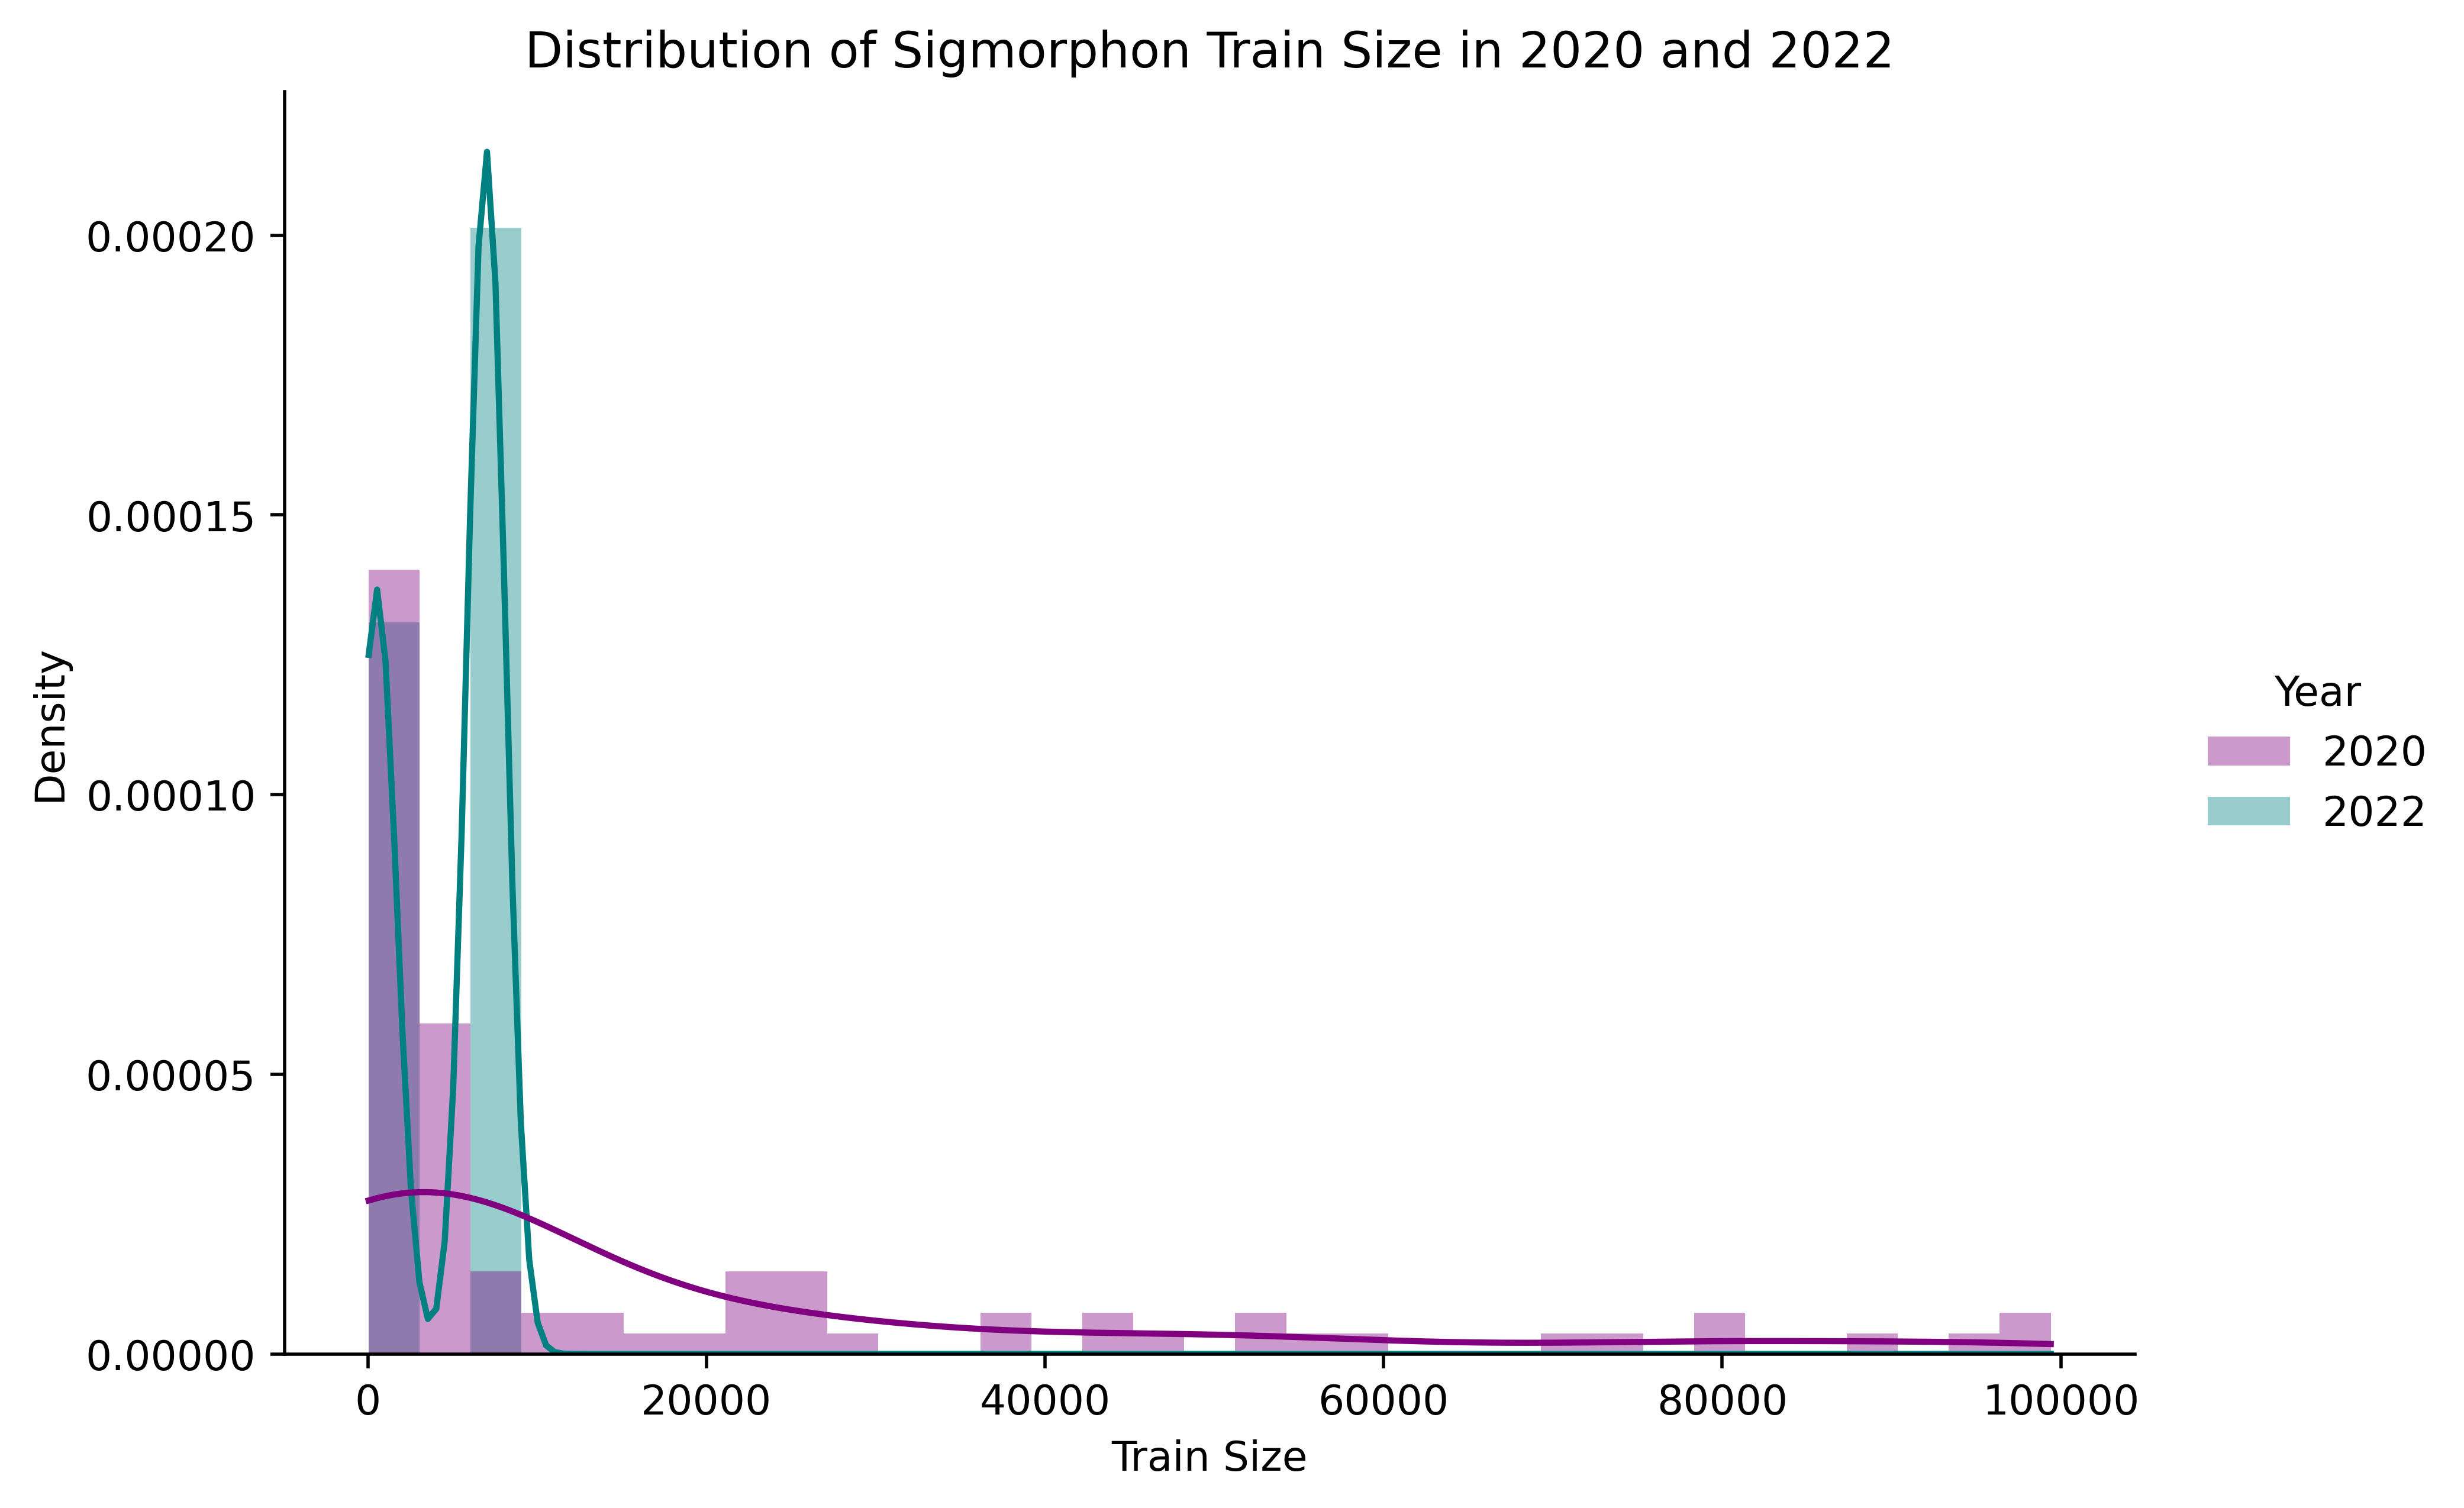
\includegraphics[width=0.8\linewidth]{figs/training_size.png}
\caption{\todo{write the caption}}
\label{fig:training_size}
\end{figure*}
\subsection{SIGMORPHON Year }

While \goldmana's data came from the 2020 SIGMORPHON shared task, \kodnera's came from the 2022 SIGMORPHON shared task. 
While SIGMORPHON 2020 contained 90 languages and SIGMORPHON 2022 contained 33, only \textit{seven} languages were shared between these years.
What's more, there is a notable difference in training size between the 2020 and 2022 versions of the shared task: while \kodnera~ capped their large training sets at 7,000 triples (smaller training sizes were used when fewer triples were available), \goldmana~ made use of the entirety of the available data, resulting in much larger training sizes on average.
Indeed, while the mean training size for \goldmana~ was 
\todo{sigmorphon, not goldman}
Mean train size in 2022: 4452.939 (stdev: 3162.846837508738)
Mean train size in 2020: 17488.933 (stdev: 26035.04482628495)

Due to this large difference in evaluation languages and training sizes, then, the results of \goldmana~ and \kodnera~ cannot be directly compared: \todo{} 



One notable difference between the SIGMORPHON shared tasks in 2020 and 2022 is with regards to training data size.

\begin{itemize}
\item Sigmorphon 2022 vs. 2020 training sizes and overlap in languages
\item The issues with the \goldmana sampling strategy 
\end{itemize}


When re-splitting, we kept the same proportions of the form-split data, we split the inflection tables: 70\%, 10\%, 20\% for the train, dev, and test sets. 
In terms of examples the proportions may vary as not all tables are of equal size. In prac- tice, the averaged train set size in examples terms was only 3.5\% smaller in the lemma-split data, on average.
\todo{look at how much of a difference there was here}
we split the inflection tables: 70\%, 10\%, 20\% for the train, dev, and test sets. 
In terms of examples the proportions may vary as not all tables are of equal size. In prac- tice, the averaged train set size in examples terms was only 3.5\% smaller in the lemma-split data, on average.

\begin{figure*}[h!]
\centering
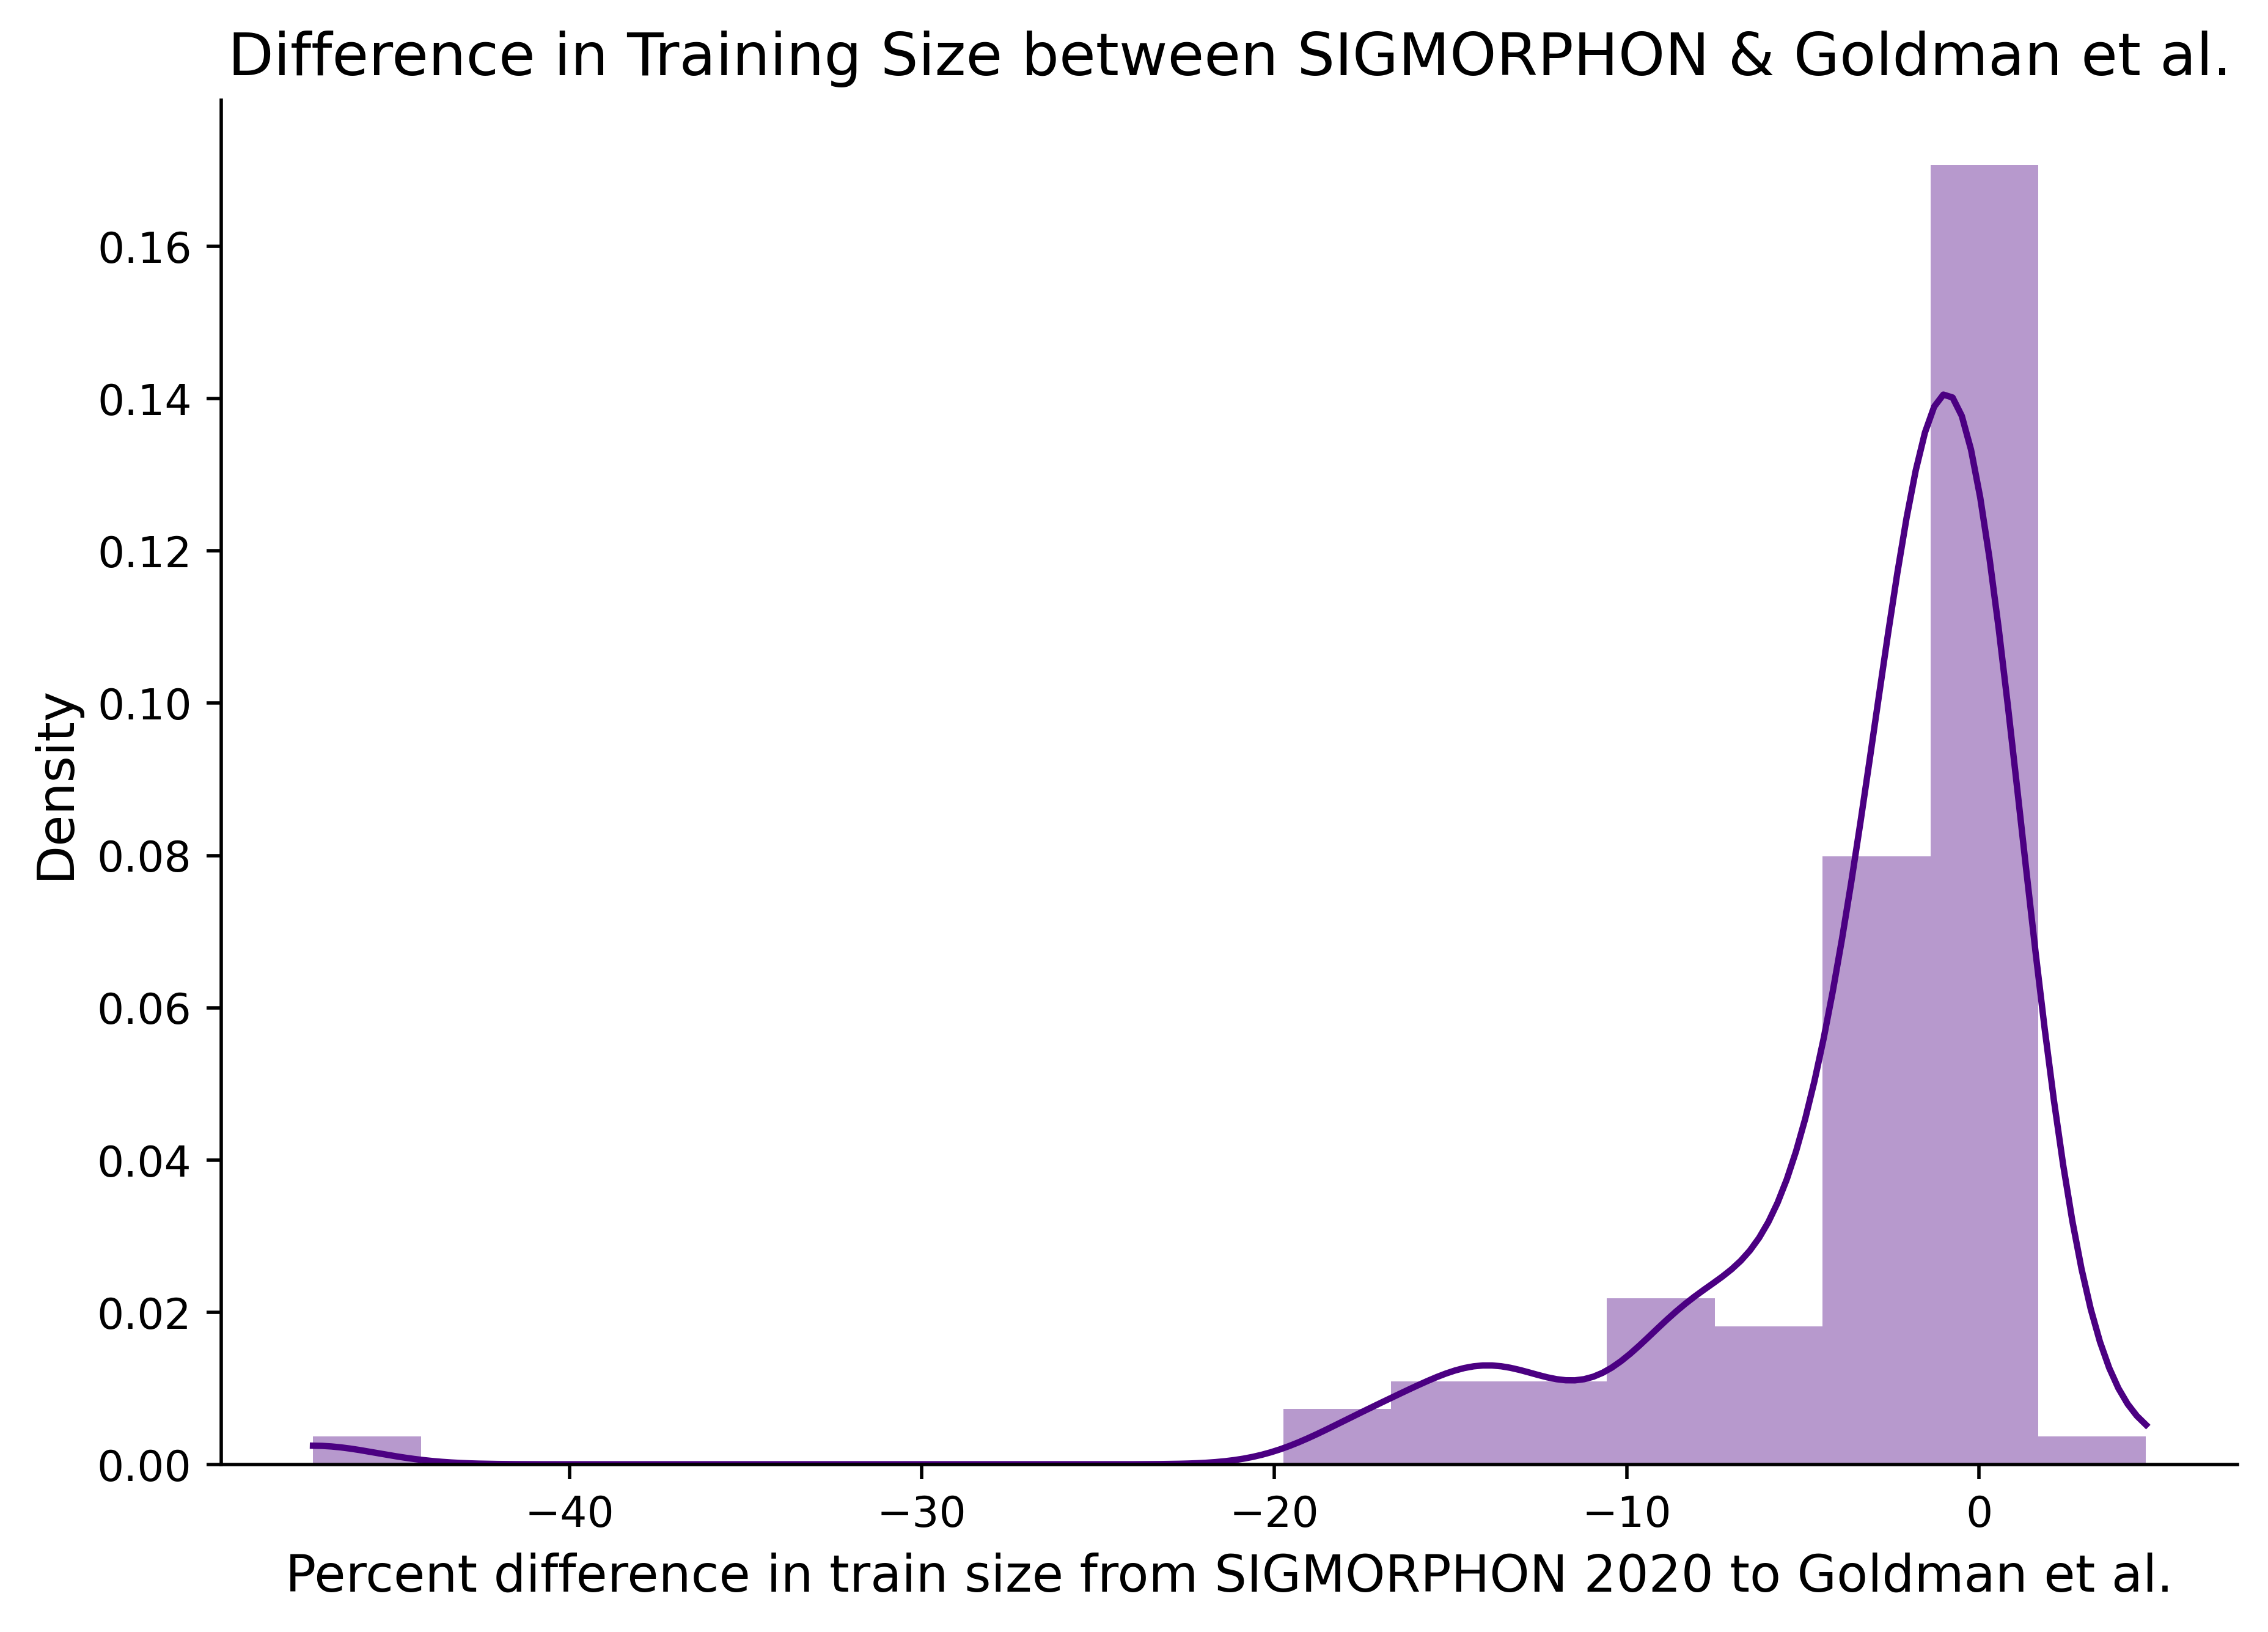
\includegraphics[width=0.8\linewidth]{figs/training_difference.png}
\caption{\todo{write the caption}}
\label{fig:training_difference}
\end{figure*}
\subsection{SIGMORPHON Year }


\subsection{Relationships Between Lemma \& Feature Set Overlap}

\begin{figure*}[h!]
\centering
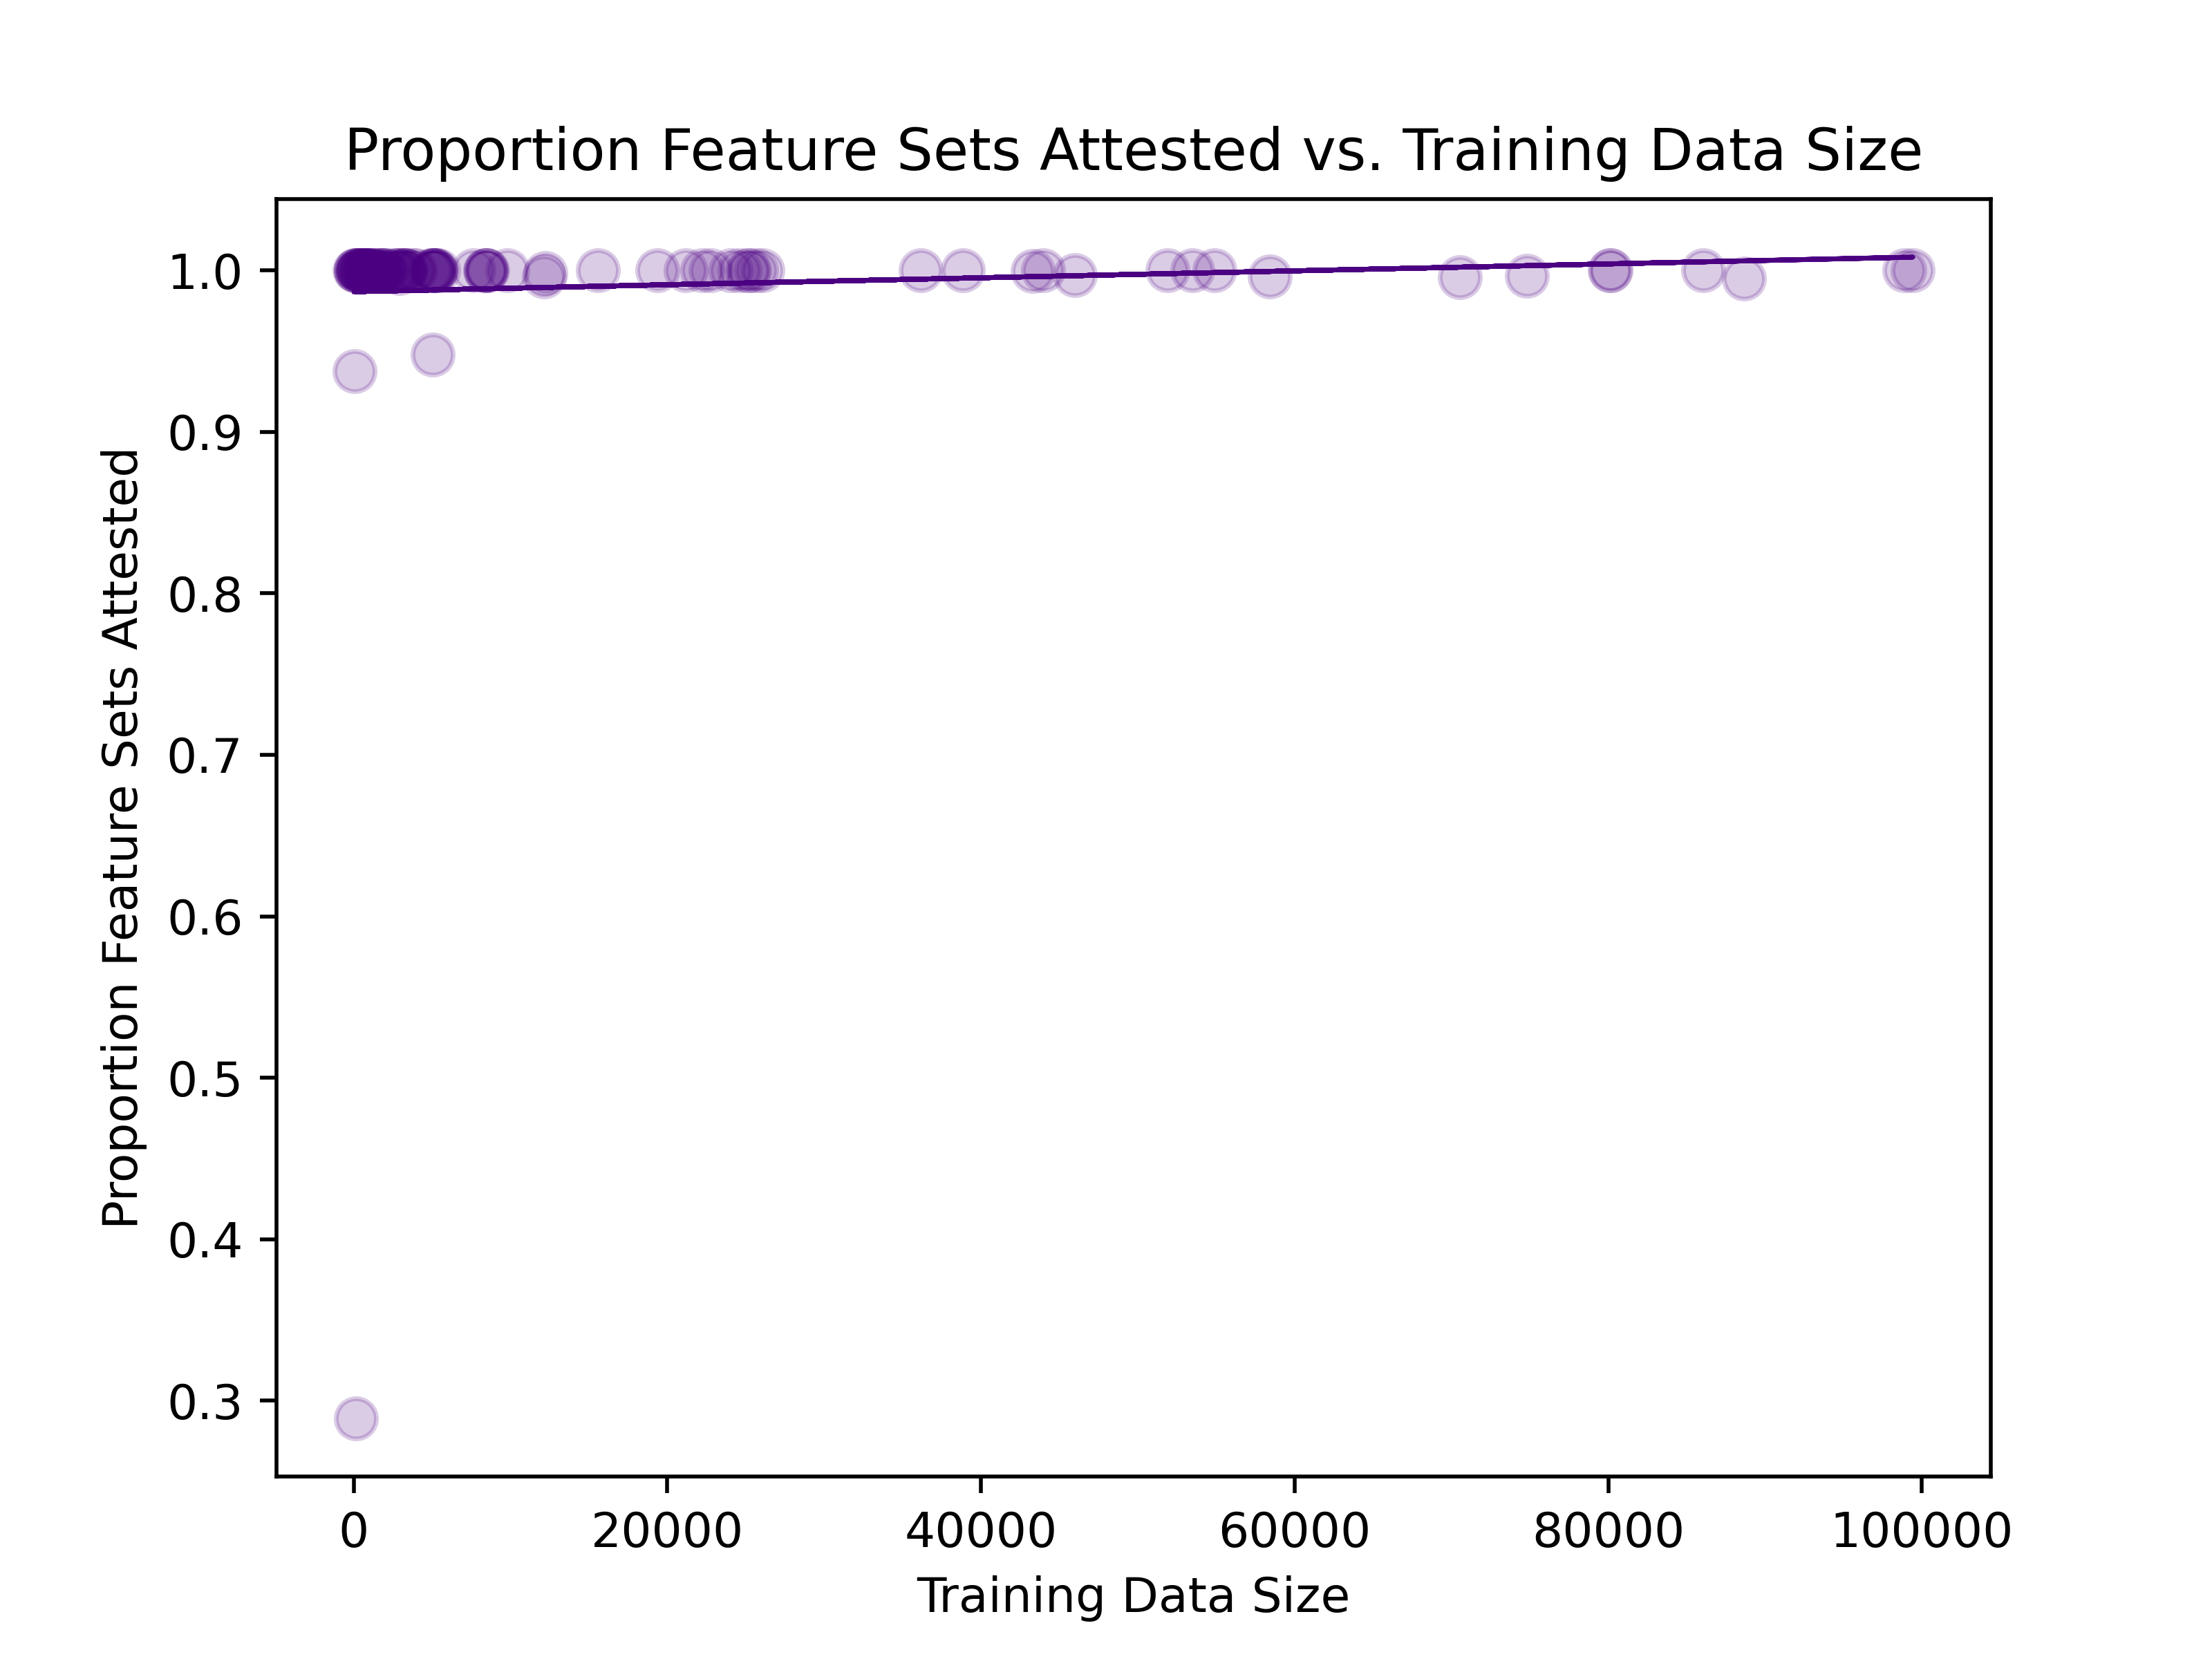
\includegraphics[width=0.8\linewidth]{figs/feats_attested.png}
\caption{The proportion of feature sets appearing in test that have been seen in train, as a function of training data size. The relationship is not significant (Pearson's $r = 0.074~(p=p = 0.489)$, Spearman's $\rho = -0.183~(p=0.084)$, Kendall's $\tau_B = -0.155~(p = 0.067)$).}
\label{fig:feats_attested}
\end{figure*}


One possible explanation for the differing results between \goldmant~ and \kodnert~ is that lemma overlap and feature set overlap are correlated, and thus that the apparent effect of lemma overlap found by \goldmana~ is \textit{actually} a result of feature set overlap.
However, under  \goldmana's lemma-based splitting, feature set overlap between train and test \textit{should} always be at ceiling: since entire paradigms are placed in either train or test, all feature sets in the test set should already be attested in train. %, so long as there is another lemma of the same part of speech in the train set. 
For example, if we split the two verbal lemmas \texttt{walk} and \texttt{run} into train (\ref{ex:train_verb}) and test (\ref{ex:test_verb}), respectively, then each verb's entire paradigm is placed in its corresponding set.
It is straightforward to see that the feature set overlap between (\ref{ex:train_verb}) and  (\ref{ex:test_verb}) is 100\%.


\begin{exe}
\ex\label{ex:train_verb} An example lemma-based train set in the style of \goldmana: \\
\begin{tabular}{lll}
\texttt{walk} & \textsc{V;Pst} & \texttt{walked}\\
\texttt{walk} & \textsc{V;Nfin} & \texttt{walk}\\
\texttt{walk} & \textsc{V;Prs;3;Sg} & \texttt{walks}\\
\end{tabular}
\ex\label{ex:test_verb}An example lemma-based evaluation set in the style of \goldmana: \\
\begin{tabular}{ll}
\texttt{run} & \textsc{V;Pst} \\
\texttt{run} & \textsc{V;Nfin} \\
\texttt{run} & \textsc{V;Prs;3;Sg}\\
\end{tabular}
\end{exe}

There are two possible caveats to this point.
Firstly, 100\% feature set overlap will only be possible if \textit{every} part of speech that appears in test also appears in train. 
However, this assumption is entirely tenable given a moderate data sample, and indeed all parts of speech appearing in the \goldmana~ test data also appear in the training data. 
Even with 100\% part-of-speech overlap, however, there is the possibility of gaps: if \texttt{stride} is the only verbal lemma in our English training data, for example, then the past participle will not be attested in train. 
Even in cases of gaps, however, it is reasonable to expect feature overlap to remain near-ceiling given moderate data given the \goldmana~ lemma-based splitting strategy. 

Indeed, when we examine the feature set overlap in the data used by \goldmana~ (Figure \ref{fig:feats_attested}), we find that the overlap for most languages is 100\%, and there is little relationship between feature set overlap and training size.
However, not all languages achieve 100\% feature set overlap:  the most dramatic outlier, Ludic, for example, has a feature overlap of just 0.303, meaning that less than a third of the feature sets appearing in the test set are attested in the train set.
Preliminary examination of the Ludic data finds that this low overlap is due to just \textit{three} of the 26 total lemmas appearing in the test data. 
One of these lemmas, \texttt{astuda} ``go", appears with a whopping 131 feature sets. 

We can ask whether it's reasonable to expect a model to generate all 131 of these feature sets by comparing the size of this test paradigm to paradigms of the same part-of-speech in train. 
In this case, \texttt{astuda}  is a verb, and the average size of a verbal paradigm in the Ludic training data is just 1.562 (stdev: 0.864); even the largest verbal paradigm contains just 16 feature sets. 
A difference of this magnitude cannot be explained simply as the result of gaps or other naturalistic phenomena. 
Rather, it seems that cases where \citeauthor{goldman-etal-2022-un}'s sampling strategy does not yield 100\% feature set overlap emerge as a result of data issues. 
Indeed, the corpus from which the Ludic data was drawn \citep{ludic} contains a large number of incomplete paradigms.
Given these conditions, it is not surprising  that the lemma-based splitting algorithm used by \goldmana~ will lead to low feature overlap. 
We investigate such issues with the data below.

\subsection{(Lack of) Data Quality}

\begin{figure*}[h!]
\centering
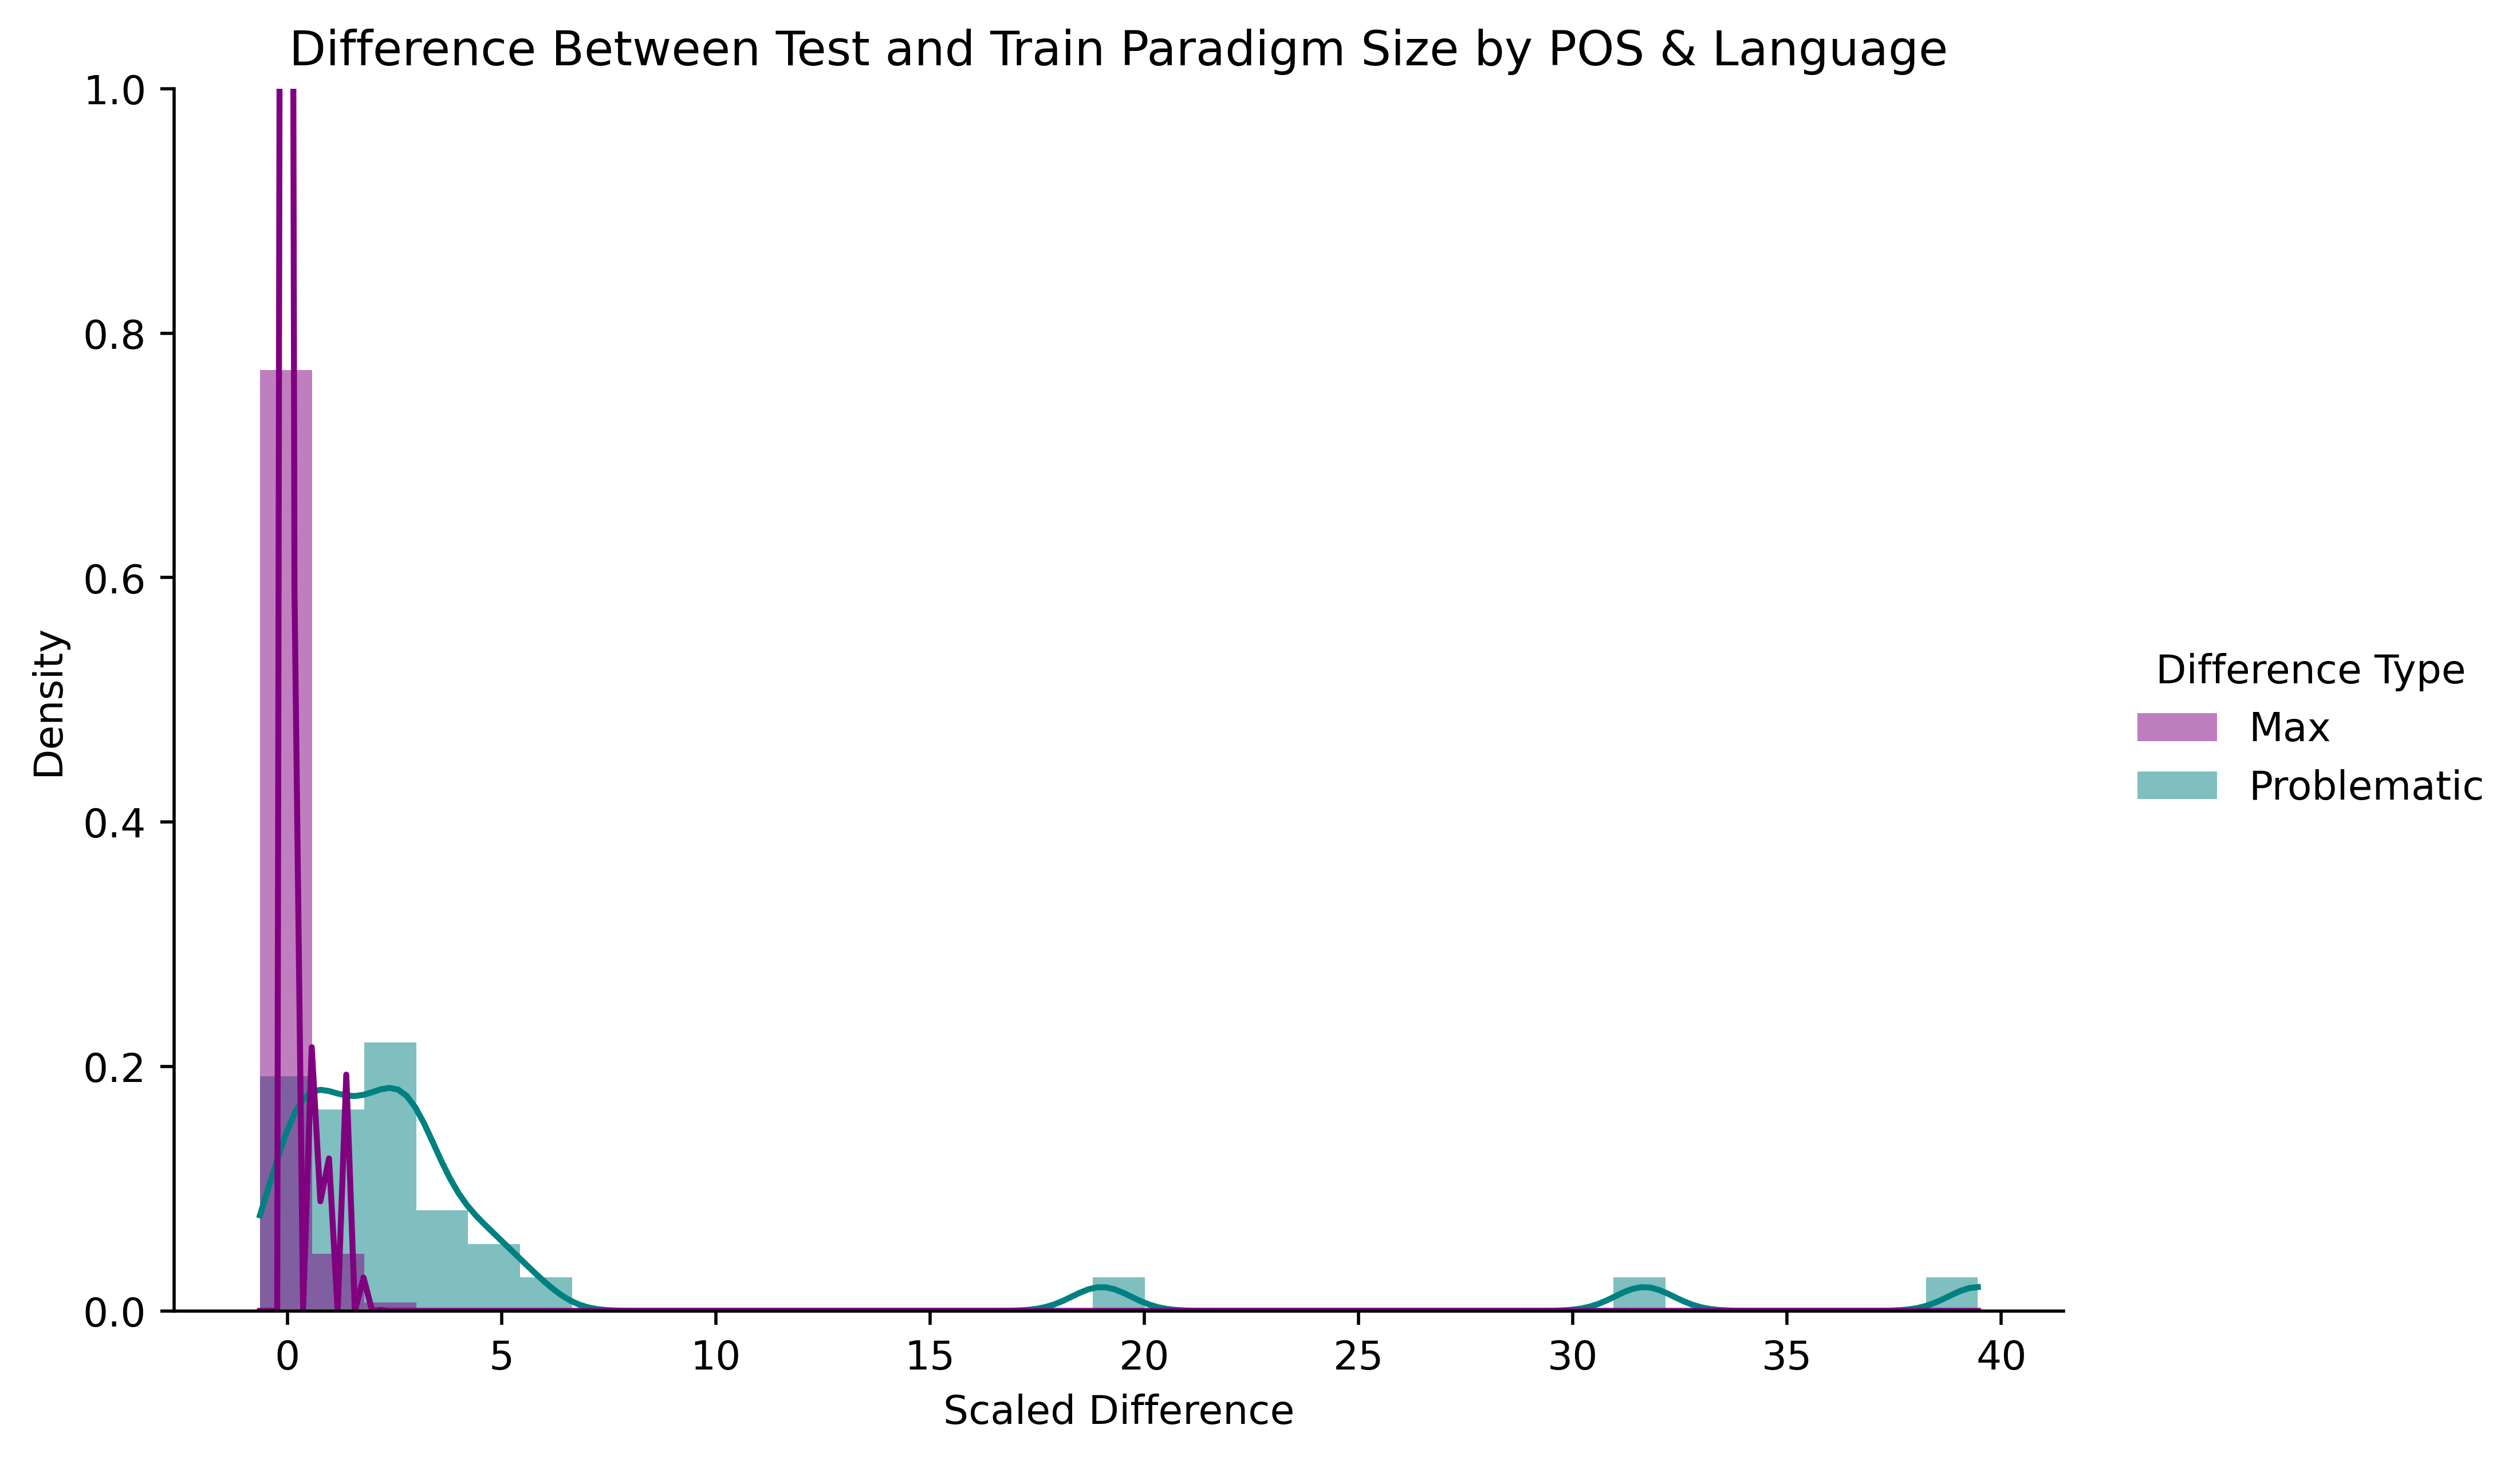
\includegraphics[width=0.8\linewidth]{figs/percent_increase.png}
\caption{The proportion of feature sets appearing in test that have been seen in train, as a function of training data size. The difference in distributions is significant (unpaired $t = 5.375,~p < 10^{-6}$).}
\label{fig:feats_attested}
\end{figure*}


Though Ludic is by far the most glaring example, the pattern of large paradigms in test causing low feature overlap  extends to other  languages for which overlap is less than 100\%. 
To quantify this, we measure the percent increase in paradigm size for  \textbf{problematic lemmas} --- those  those appearing with at least one unattested feature set in test --- compared to the average paradigm size of words with the same part of speech in the training data.
In other words, we calculate:
\begin{equation}
\begin{small}
\textsc{Diff} = 100* \frac{\texttt{mean}(\textsc{ProbLem}) - \texttt{mean}(\textsc{Train})}{\texttt{mean}(\textsc{Train})}
\end{small}
\end{equation} 
Where \textsc{ProbLem} indicates the paradigm size of the problematic lemmas and \textsc{Train} indicates the paradigm size of the same POS in train. 

Indeed, we find that the mean percent difference in paradigm size between the problematic lemmas and the corresponding train lemmas is a whopping 437.683\% (stdev: 871.027\%), with the large standard deviation resulting from a number of large positive outliers. 
To give a point of comparison, we also measure the percent increase from the average training paradigm size to the \textit{maximum} test paradigm size across all POS for all languages for which there is 100\% overlap. 
Here, the mean percent increase is only 11.511\% (stdev: 34.054\%); indeed, an unpaired T-test finds a significant difference between these two measures of increase ($t = 5.375,~p < 10^{-6}$)
The difference in these distributions is visualized in Figure \ref{fig:feats_attested}.





\subsection{Model Types}
\subsection{Splitting Strategy}












\newpage






% Bibliography entries for the entire Anthology, followed by custom entries
\bibliography{anthology,custom}
% Custom bibliography entries only
%\bibliography{custom}

%\appendix
%
%\section{Example Appendix}
%\label{sec:appendix}
%
%This is an appendix.

\end{document}
